
\documentclass[10pt]{article}
\usepackage[utf8]{inputenc}
\usepackage{kotex}
\usepackage{graphicx}
\usepackage{subfigure}
\usepackage{titling}
\setlength{\droptitle}{-2cm}
\usepackage{array}
\usepackage{amssymb}
\usepackage{amsmath}
\usepackage{siunitx} 
\usepackage{enumerate} 
\usepackage{pgfplots}
\usepackage{pgfplotstable}
\usepackage{tikz,pgfplots}
\usepackage{wasysym}
\usepackage{geometry}
\usepackage{authblk}
\usepackage{kotex}
\usepackage{bibunits}
\usepackage{tabularx}
\usepackage{hyperref}
\usepackage{pythonhighlight}

\geometry{
    a4paper,
    total={170mm,257mm},
    left=20mm,
    top=20mm,
}

\title{\textbf{Mathematical Foundation of DNN : HW 10}}
\author{Jeong Min Lee}

\begin{document}
\maketitle

\section*{1}
\begin{align*}
    &\nabla_{\phi} \mathbb{E}_{Z\sim q_{\phi}(z)}\left[\log \left(\frac{h(Z)}{q_{\phi}(Z)}\right)\right] \\
    &= \nabla_{\phi}\int dz \log \left(\frac{h(z)}{q_{\phi}(z)}\right)q_{\phi}(z) \\
    &= \nabla_{\phi} \int dz\ q_{\phi}(z)\log h(z) - q_{\phi} (z)\log q_{\phi}(z) \\ 
    &= \int dz \ \left(\nabla_\phi q_\phi(z)\right) \log h(z) - \left(\nabla_\phi q_\phi(z)\right) \log q_{\phi}(z) - q_\phi(z) \nabla_\phi \log q_\phi(z)\\
    &= \int dz \ \left(\nabla_\phi q_\phi(z)\right) \log h(z) - \left(\nabla_\phi q_\phi(z)\right) \log q_{\phi}(z) - \nabla_\phi q_\phi(z) \\
    &= \int dz \ \nabla_\phi q_\phi(z)\log \left(\frac{h(z)}{q_\phi(z)}\right) - \int dz \ \nabla_\phi q_\phi(z) \\
    &= \int dz \ q_\phi \nabla_\phi \log q_\phi(z) \log \left(\frac{h(z)}{q_\phi(z)}\right) \\
    &= \mathbb{E}_{Z \sim q_\phi}\left[\left(\nabla_\phi \log q_\phi(z)\right) \log \left(\frac{h(z)}{q_\phi(z)}\right)\right]
\end{align*}
\section*{2}
\begin{align*}
    \Pi_C(y) &= \underset{x\in C}{\arg\min} \lVert x - y \rVert^2 \\
    &= \underset{0 \le x_2 \le 1}{\arg\min} \bigg\lVert \begin{pmatrix}
        a-y_1 \\ x_2 - y_2
    \end{pmatrix}\bigg\rVert^2 \\
    &= \underset{0 \le x_2 \le 1}{\arg\min} (a-y_1)^2 + (x_2 - y_2)^2 \\
    &= \begin{pmatrix} a \\ \underset{0 \le x_2 \le 1}{\arg\min} (x_2 - y_2)^2 \end{pmatrix}
\end{align*}

\begin{figure}[!h]
    \begin{center}
        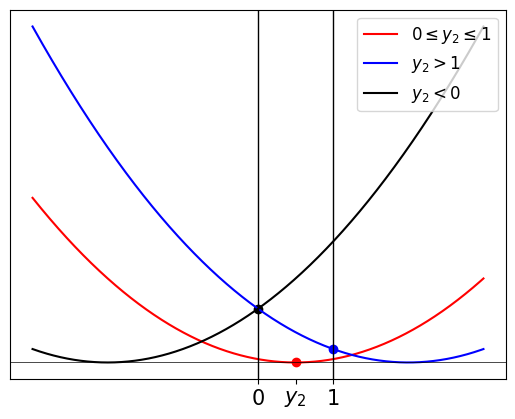
\includegraphics[scale = 0.5]{../hw10/fig1.png}
    \end{center}
    \caption{$\Pi_C(y)$ accroding to the value of $y_2$. The bold dots denote the minimum value for each case.}
    \label{fig1}
\end{figure}

According to the figure \ref{fig1}, the minimal value of $(x_2 - y_2)^2$ depends on the range of $y_2$.
\begin{equation}
    \underset{0 \le x_2 \le 1}{\arg\min} (x_2 - y_2)^2 = \begin{cases}
        0 \text{ if } y_2 <0 \\
        y_2 \text{ if } 0 \le y_2 \le 1 \\
        1 \text{ if }y_2 >1
    \end{cases}
    \label{eqn1}
\end{equation}

To sum up, one can observe that the equation \ref{eqn1} can be simplified by $\min\left\{\max \left\{y_2, 0\right\},1\right\}$. 
Thus, proof is done. 
\section*{3}
The following code is the implementation of image inpainting with flow model. 
I used negative of maximum likelihood as a loss and enforced the conditions on $X$ for each iteration by using clipping.
Note that I used SGD as an optimizer, not an Adam. The results of the following code are listed on the figure \ref{fig2}.
\begin{python}
... 

lr = 1e-3

X = image.clone().requires_grad_(True)

# Set optimizer
optimizer = torch.optim.SGD([X], lr=lr)

# Define the inpainting loop that projects the gradients and performs the update
for i in range(300):
    optimizer.zero_grad()
    loss = -model(X.view(1, -1))
    loss.backward()
    optimizer.step()

    with torch.no_grad():
        X.data = torch.clamp(X.data, min = 0, max = 1)
        X.data[mask] = image.data[mask]

recon = X.detach().view(1, 28, 28)
# Plot reconstruction
plt.figure(figsize = (4,4))
plt.title('Reconstruction')
plt.imshow(make_grid(recon.squeeze().detach()).permute(1,2,0))
# plt.show()
plt.savefig('plt3.png')
\end{python}

\begin{figure}[!h]
    \begin{center}
        \subfigure[]{
            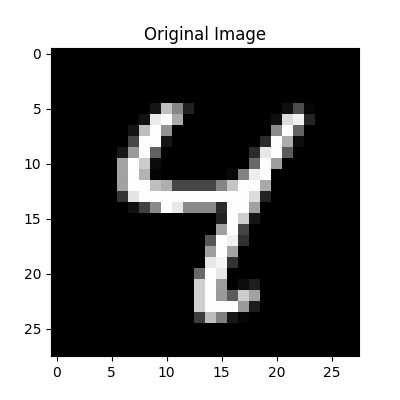
\includegraphics[scale = 0.3]{../hw10/plt1.png}
        }
        \subfigure[]{
            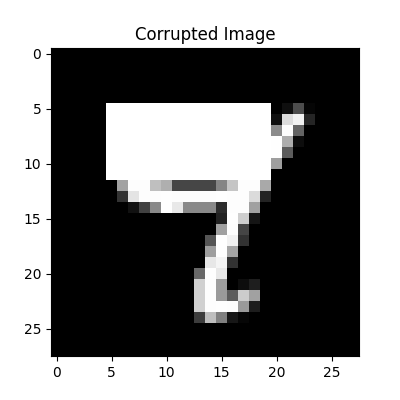
\includegraphics[scale = 0.3]{../hw10/plt2.png}
        }
        \subfigure[]{
            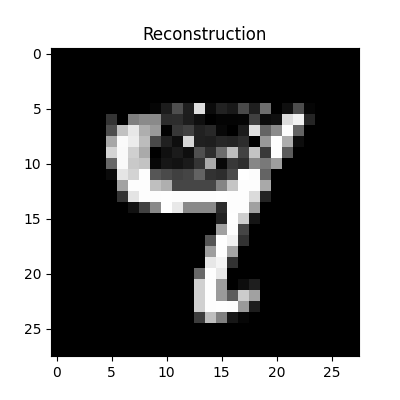
\includegraphics[scale = 0.3]{../hw10/plt3.png}
        }
    \end{center}
    \caption{(a) Orinal Image, (b) Corrupted Image, (c) Reconstructed image by using an algorithm above.}
    \label{fig2}
\end{figure}

\section*{4}
\subsection*{a}
\begin{equation}
    {\partial f_1 \over \partial x} = A
    \label{eqn2}
\end{equation}
According to the equation \ref{eqn2}, $\left|{\partial f_1 / \partial x} \right| = \left| \det{({\partial f_1 / \partial x})} \right| = \left| \det A\right|$.
\begin{align*}
    \det A &= \det PL(U + \text{diag}(s)) \\
    &= \det P \det L \det(U + \text{diag}(s)) \\
    &= \det(U + \text{diag}(s)) (\because \det P = \det L = 1) \\
    &= \prod_{i=1}^C s_i
\end{align*}
Thus, $\log \left|{\partial f_1 / \partial x} \right| = \log \left|\prod_{i=1}^C s_i\right| = \sum_{i=1}^C \log |s_i|$.
\subsection*{b}
Define $h(X)$ as follow.
\begin{equation}
    h(X) = \left[\begin{pmatrix}
        h(X_{111}) & \cdots & h(X_{11c}) \\
        \vdots & \ddots & \vdots \\ 
        h(X_{1b1}) & \cdots & h(X_{1bc})
    \end{pmatrix}, \cdots, \begin{pmatrix}
        h(X_{a11}) & \cdots & h(X_{a1c}) \\
        \vdots & \ddots & \vdots \\ 
        h(X_{ab1}) & \cdots & h(X_{abc})
    \end{pmatrix} \right]
\end{equation}
Also, defined the following reshape as standard reshape. 
\begin{align}
    \left[\begin{pmatrix}
        h(X_{111}) & \cdots & h(X_{11c}) \\
        \vdots & \ddots & \vdots \\ 
        h(X_{1b1}) & \cdots & h(X_{1bc})
    \end{pmatrix}, \cdots, \begin{pmatrix}
        h(X_{a11}) & \cdots & h(X_{a1c}) \\
        \vdots & \ddots & \vdots \\ 
        h(X_{ab1}) & \cdots & h(X_{abc})
    \end{pmatrix} \right] \\ \longrightarrow \left[ h(X_{111}), h(X_{112}), \cdots, h(X_{11c}), h(X_{121}), \cdots, h(X_{12c}), \cdots, h(X_{abc})\right]
\end{align}

Note that the mapping from $(i,j,k) \rightarrow l = (i-1)bc + (j-1)c + k$, is the mapping from $h(X)_{ijk}$ to $[h(X).reshape(abc)]_l$.
Although there are a $(abc)!$ number of reshape from $\mathbb{R}^{a\times b\times c} \rightarrow \mathbb{R}^{abc}$, noting inherent feature of reshape, that is reshape is enumeration of matrix elements in a 1D array,
an permuation from $\left\{1, 2, ..., abc\right\} \rightarrow \left\{1, 2, ..., abc\right\}$ that make each reshape of $h(X)$ identical to standard reshape trivially exists. 
The formalization of this statement is following: $\exists P\in \mathbb{R}^{abc \times abc} \text{ s.t. } P(h(X).reshape(abc)) = h(X).standard\_reshape(abc)$.
Thus, for each reshape rule, there is permutation matrix $P$ where the equation \ref{eqn6} holds
\begin{equation}
    {\partial h(X).reshape(abc) \over \partial X.reshape(abc)} = P{\partial h(X).standard\_reshape(abc) \over \partial X.standard\_reshape(abc)}P^{-1}
    \label{eqn6}
\end{equation}
Since the permutation matrix $P$ has the determinant of 1, one can conclude the absolute value of the Jacobian determinant with vectorization is well defined. 
\subsection*{c}
\begin{align*}
    \left[f_2(X|P,L,U,s)\right]_{ijk} &= \sum_{l=1}^C w_{i,l,1,1}X_{ljk} \\
    &= \sum_{l=1}^{C}A_{il}X_{ljk} \\
    {\partial \over \partial X_{mnl}} f_2(X|P,L,U,s)_{ijk} &= \sum_{r=1}^C {\partial \over \partial X_{mnl}} A_{ir}X_{rjk} \\
    &= \sum_{r=1}^C A_{ir}\delta_{mr}\delta_{jn}\delta_{lk} \\
    &= A_{im}\delta_{jn}\delta_{lk}
\end{align*}
The Kronecker delta symobl implies that the ${\partial f_2(X|P,L,U,s)}/ \partial X$ is kind of diagonal tensor, which enforce $j = n, l = k$ like to diagonal matrix. 
Also, note that ${\partial f_2(X|P,L,U,s)_{:,j,k}}/ \partial X_{:,j,k} = A$.
The determinant of diagonal matrix is identical to the product of all diagonal entries, or the determinant of diagonal entries(The determinant of scalar is itself.).
Likewise, the determinant of diagonal tensor is the product of all diagonal tensor's determinant.  
In this case, $A$ acts as an diagonal element of the Jacobian.\footnote{Here the Jacobian is diagonal with respect to $(j,n), (l,k)$ and the diagonal element is defined the element where $j = n, l = k$. This can be clear when considering the case of diagonal matrix. A matrix $P$ is diagonal w.r.t $(i,j)$ if and only if $P_{ij} = p_i\delta_{ij}$ and the diagnal element of $P$ is the element where $i=j$.}
Thus, the determinant of Jacobian is $mn$ number of product of $\det A$.
\begin{equation}
    \left|{\partial \over \partial X} f_2(X|P,L,U,s)\right|  = \left|\det A\right|^{mn}
\end{equation}
Thus, $ \log \left|{\partial f_2(X|P,L,U,s) / \partial X} \right| = \log  \left|\det A\right|^{mn} = mn \log \left|\det A\right| = mn \sum_{i=1}^C\log|s_i|$.
\subsection*{d}
\begin{equation}
    Z_{1:C,:,:} = X_{1:C,:,:}
\end{equation}
\begin{equation}
    Z_{C+1:2C,:,:} = f_2(X_{C+1:2C,:,:}|P, L(X_{1:C,:,:}), U(X_{1:C,:,:}),s(X_{1:C,:,:}))
    \label{eqn9}
\end{equation}
Considering the definition of $Z$ as above, $\partial Z /\partial X$ has block lower triangular matrix as follow.
\begin{align*}
    {\partial Z \over \partial X} &= \begin{pmatrix}
        {\partial Z_{1:C,:,:} \over \partial X_{1:C,:,:}} & {\partial Z_{1:C,:,:} \over  \partial X_{C+1:2C,:,:}} \\
        {\partial Z_{C+1:2C,:,:} \over \partial X_{1:C,:,:}} & {\partial Z_{C+1:2C,:,:} \over \partial X_{C+1:2C,:,:}}
    \end{pmatrix} \\
    &= \begin{pmatrix}
        \boldsymbol{1}_{C} & 0 \\
        \star & {\partial Z_{C+1:2C,:,:} \over \partial X_{C+1:2C,:,:}}
    \end{pmatrix}
\end{align*}
Thus, $\det {\partial Z / \partial X} = \det {\partial Z_{C+1:2C,:,:} / \partial X_{C+1:2C,:,:}}$, and due to equation \ref{eqn9}, 
\begin{equation}
   \log \left(\left| {\partial Z_{C+1:2C,:,:} \over \partial X_{C+1:2C,:,:}}\right|\right) =\log\left( \left|\partial {f_2(X_{C+1:2C,:,:}|P, L(X_{1:C,:,:}), U(X_{1:C,:,:}),s(X_{1:C,:,:}))\over \partial X_{C+1:2C,:,:}}\right|\right) = mn \sum_{i=1}^C\log |s_i|
\end{equation}
Note that the last equation is followed by the problem 4-(c).

\section*{5}
The following code is implementation to calculate the probability that gambler leave the casino with \$200 with Monte Carlo simulation.
The Estimated probability of reaching \$200 before going broke was about 2.756788395553154e-6.

\begin{python}
import numpy as np

# Set the parameters
p = 18 / 37  # Probability of winning
q = 0.55     # Importance sampling probability (q > p)
initial_balance = 100
goal = 200
num_simulations = 3000
max_games = 600

def run_simulation(p, q, initial_balance, goal, max_games):
    balance = initial_balance
    weight = 1.0  # Initialize the weight for importance sampling
    
    for _ in range(max_games):
        # Simulate a game with the importance sampling distribution
        if np.random.rand() < q:
            balance += 1  # Win
            weight *= p / q  # Update the weight
        else:
            balance -= 1  # Lose
            weight *= (1 - p) / (1 - q)  # Update the weight
        if balance == 0 or balance == goal:
            break
        return balance == goal, weight

results = [run_simulation(p, q, initial_balance, goal, max_games) for _ in range(num_simulations)]

probability_estimate = sum(weight for success, weight in results if success) / num_simulations
print(f'Estimated probability of reaching ${goal} before going broke: {probability_estimate}')

\end{python}
\section*{6}
\subsection*{a}
To implement the following code, I calculated the gradient of objective function. 
\begin{align*}
    &\nabla_{\mu, \sigma^2} \mathbb{E}\left[X \sin X\right] + \frac{1}{2}(\mu - 1)^2 + \sigma - \log \sigma \\
    &= \begin{pmatrix}
        {\partial \over \partial \mu} \mathbb{E}\left[X \sin X\right]  + \mu -1 \\
        {\partial \over \partial \sigma} \mathbb{E}\left[X \sin X\right]  + 1  - 1/\sigma
    \end{pmatrix} \\
    &=  \begin{pmatrix}
        \mathbb{E}\left[X \sin X {\partial \over \partial \mu } \log f \right]  + \mu -1 \\
       \mathbb{E}\left[X \sin X  {\partial \over \partial \sigma} \log f \right]  + 1  - 1/\sigma 
    \end{pmatrix} \text{ where } f(x) = \frac{1}{\sqrt{2\pi \sigma^2}}e^{-(x-\mu)^2/2\sigma^2} 
\end{align*}
By inserting followin derivatives into the equation above, the gradient of objective function can be derived.
\begin{align*}
    {\partial \over \partial \mu } \log f &= \frac{x-\mu}{\sigma^2}\\
    {\partial \over \partial \sigma } \log f &= \frac{(x-\mu)^2}{\sigma^2} - 1/\sigma^2
\end{align*}
\begin{python}
mu = 0
tau = 0
B = 32
lr = 1e-1
iteration = 500

logger = []

def loss(X, mu, tau):
    return torch.sum(X*torch.sin(X))/X.shape[0] + 0.5*(mu-1)**2 + np.exp(tau) - tau

for _ in range(iteration):
    X = np.exp(tau)*torch.normal(0,1,size=(B,1)) + mu
    g1 = torch.sum(X*torch.sin(X)*((X-mu)/np.exp(2*tau)))/B + mu -1
    g2 = torch.sum(X*torch.sin(X)*(-1 + (X-mu)**2*np.exp(-2*tau)))/B + np.exp(tau)-1
    mu -= lr*g1/B
    tau -=lr*g2/B
    logger.append(loss(X, mu, tau))

plt.plot(range(iteration),logger)
plt.xlabel("Iteration")
plt.ylabel("Loss")

print(mu.item())
print(np.exp(tau.item()))

\end{python}
\begin{python}
0.4434947967529297
0.6487261602209319
\end{python}
\subsection*{b}
According to the definition of Gaussian random variable, if $Y\sim \mathcal{N}(0,1)$, the derived random variable $X = \sigma Y + \mu$ is the Gaussian random variable with mean $\mu$, variance $\sigma^2$. Thus, from the reparametrization trick, 
\begin{align*}
    &\nabla_{\mu, \sigma^2} \mathbb{E}_{X\sim \mathcal{N}(\mu, \sigma^2)}\left[X \sin X\right] + \frac{1}{2}(\mu - 1)^2 + \sigma - \log \sigma \\
    &= \nabla_{\mu, \sigma^2} \mathbb{E}_{X\sim \mathcal{N}(\mu, \sigma^2)}\left[X \sin X \right] + \nabla_{\mu, \sigma^2} \frac{1}{2}(\mu - 1)^2 + \sigma - \log \sigma\\  
    &= \mathbb{E}_{Y\sim \mathcal{N}(0,1)}\left[\left(\sin X + X\cos X, (\sin X + X\cos X) Y\right)^T\right] + (\mu-1, 1 - 1/\sigma)^T
\end{align*}
\begin{python}
mu = 0
tau = 0
B = 32
lr = 1e-2
iteration = 500

logger = []

def loss(X, mu, tau):
    return torch.sum(X*torch.sin(X))/X.shape[0] + 0.5*(mu-1)**2 + np.exp(tau) - tau

for _ in range(iteration):
    Y = torch.normal(0,1,size=(B,1))
    sigma = np.exp(tau)
    X = mu + sigma*Y
    g1 = torch.sum(torch.sin(X) + X*torch.cos(X))/B + mu-1
    g2 = torch.sum((torch.sin(X) + X*torch.cos(X))*sigma*Y)/B + sigma - 1

    mu -= lr*g1
    tau -=lr*g2

    logger.append(loss(X, mu, tau))

plt.plot(range(iteration),logger)

print(mu.item())
print(np.exp(tau.item()))
\end{python}
\begin{python}
0.44522392749786377
0.6097483273335648
\end{python}


\end{document}